\everymath{\displaystyle}
\documentclass{beamer}
% \documentclass[handout]{beamer}

%\usepackage[pdftex]{color,graphicx}
\usepackage{amsmath,amssymb,amsfonts}

\mode<presentation>
{
  % \usetheme{Darmstadt}
  % \usetheme[hideothersubsections]{Hannover}
  % \usetheme[hideothersubsections]{Goettingen}
  \usetheme[hideothersubsections, right]{Berkeley}

  \usecolortheme{seahorse}
  % \usecolortheme{dolphin}
  \usecolortheme{rose}
  % \usecolortheme{orchid}

  \useinnertheme[shadow]{rounded}

  % \setbeamercovered{transparent}
  \setbeamercovered{invisible}
  % or whatever (possibly just delete it)
}

\mode<handout>{
  \setbeamercolor{background canvas}{bg=black!5}
  \usepackage{pgfpages}
  \pgfpagesuselayout{4 on 1}[a4paper,border shrink=5mm, landscape]
}

\usepackage[brazilian]{babel}
% or whatever

% \usepackage[latin1]{inputenc}
\usepackage[utf8]{inputenc}
% or whatever

\usepackage{times}
%\usepackage[T1]{fontenc}
% Or whatever. Note that the encoding and the font should match. If T1
% does not look nice, try deleting the line with the fontenc.


\title%[] % (optional, use only with long paper titles)
{Comparação de dois grupos (qualitativo)}

\subtitle
{Testes para proporções} % (optional)

\author%[] % (optional, use only with lots of authors)
{Felipe Figueiredo}% \and S.~Another\inst{2}}
% - Use the \inst{?} command only if the authors have different
%   affiliation.

\institute[INTO] % (optional, but mostly needed)
{Instituto Nacional de Traumatologia e Ortopedia
}
  % \inst{1}%
  % Department of Computer Science\\
  % University of Somewhere
  % \and
  % \inst{2}%
  % Department of Theoretical Philosophy\\
  % University of Elsewhere}
% - Use the \inst command only if there are several affiliations.
% - Keep it simple, no one is interested in your street address.

\date%[] % (optional)
{}

% \subject{Talks}
% This is only inserted into the PDF information catalog. Can be left
% out. 



% If you have a file called "university-logo-filename.xxx", where xxx
% is a graphic format that can be processed by latex or pdflatex,
% resp., then you can add a logo as follows:

\pgfdeclareimage[height=1.6cm]{university-logo}{../logo}
\logo{\pgfuseimage{university-logo}}



% Delete this, if you do not want the table of contents to pop up at
% the beginning of each subsection:
\AtBeginSubsection[]
%\AtBeginSection[]
{
  \begin{frame}<beamer>{Sumário}
    \tableofcontents[currentsection,currentsubsection]
  \end{frame}
}


% If you wish to uncover everything in a step-wise fashion, uncomment
% the following command: 

% \beamerdefaultoverlayspecification{<+->}

\usepackage[normalem]{ulem}

\begin{document}

\begin{frame}
  \titlepage
\end{frame}

\begin{frame}{Sumário}
  \tableofcontents
  % You might wish to add the option [pausesections]
\end{frame}


%% Template
% \section{}

% \subsection{}

% \begin{frame}{}
%   \begin{itemize}
%   \item 
%   \end{itemize}
% \end{frame}

% \begin{frame}
%   \begin{columns}
%     \begin{column}{5cm}
%     \end{column}
%     \begin{column}{5cm}
%     \end{column}
%   \end{columns}
% \end{frame}

% \begin{frame}{}
%   \includegraphics[height=0.4\textheight]{file1}
%   \includegraphics[height=0.4\textheight]{file2}
%   \includegraphics[height=0.4\textheight]{file3}
%   \begin{figure}
%     \caption{}
%   \end{figure}
% \end{frame}

% \begin{frame}{}
%   \begin{definition}
%   \end{definition}
%   \begin{example}
%   \end{example}
%   \begin{block}{Exercício}
%   \end{block}
% \end{frame}

\section{Discussão da aula passada}

\subsection{Discussão da aula passada}

\begin{frame}{Discussão da aula passada}
  \begin{block}{}
    Discussão da leitura obrigatória da aula passada
  \end{block}
\end{frame}

\section[1 amostra]{Observação x expectativa (1 amostra)}

\subsection{Objetivo da aula}

\begin{frame}{Dados categóricos}
  \begin{itemize}
  \item Vamos analisar contagens de dados categóricos (ou nominais)
  \item Para estas variáveis qualitativas não existe ordenação interente
  \item Observamos apenas as contagens e frequências destes dados em
    uma amostra.
  \end{itemize}
  \begin{exampleblock}{Exemplo}
    doente/sadio, fumante/não fumante, masculino/feminino, olhos
    castanhos/olhos azuis/olhos verdes, etc.
  \end{exampleblock}
\end{frame}

\begin{frame}{Objetivo}
  \small
  Considere a seguinte tabela:
  \begin{exampleblock}{Exemplo}
    \footnotesize
    \begin{tabular}{c|c|c}
                 & Lesão & Não tem lesão\\
      \hline
      Alongou-se & 18 & 22\\
      \hline
      Não se alongou & 211 & 189\\
    \end{tabular}

    \bigskip
    {\hfill \scriptsize (Fonte: Larson \& Farber 2013)}
  \end{exampleblock}
  \vfill
  \begin{block}{Pergunta}
    Como determinar se existe alguma relação entre as variáveis?

    \bigskip
    \small
    Isto é: o desfecho é independente da exposição?
  \end{block}
\end{frame}

\begin{frame}{Quais são as variáveis?}
  \begin{itemize}
    \small
  \item Dependente: desfecho (categórica)
  \item Independente: exposição (categórica)
  \end{itemize}
  \vfill
  \begin{block}{Esta relação pode ser expressa como}
    \begin{displaymath}
      \text{desfecho} \sim \text{exposição}
    \end{displaymath}
  \end{block}
\end{frame}

\begin{frame}{}
  \begin{center}
    Mas antes vamos ver o caso de uma única variável.
  \end{center}
\end{frame}

\subsection{Analisando dados de contagens}

\begin{frame}{Exemplo}
  \begin{exampleblock}{Exemplo}
    Considere que 10\% dos pacientes morrem após uma operação
    arriscada. Em uma amostra de 75 pacientes, observou-se que 16
    pacientes morreram após a operação.

    Como comparar o número de óbitos osbervado e o número esperado?

    Fonte: Motulsky, 1995
  \end{exampleblock}
  \begin{itemize}
  \item O número observado de óbitos em 75 pacientes foi 16.
  \item O número esperado seria $75 \times 10\% = 7.5$
  \item A discrepância nos óbitos foi $16-7.5 = 8.5$
  \end{itemize}
\end{frame}

\begin{frame}{Quais são as variáveis?}
  \begin{itemize}
    \small
  \item Dependente: mortalidade (categórica)
  \item Independente: parâmetro fixo
  \end{itemize}
  \vfill
  \begin{block}{Esta relação pode ser expressa como}
    \begin{displaymath}
      \text{mortalidade} \sim \text{10\%}
    \end{displaymath}
  \end{block}
\end{frame}

\begin{frame}{Questões}
  \begin{itemize}
  \item Esse aumento reflete uma mudança real na mortalidade?
  \item Em uma amostra qualquer com 75 pacientes esperaríamos observar $7.5$ óbitos
  \item Em uma amostra específica poderíamos observar mais ou menos
    que isso
  \item Provavelmente algo próximo de $7.5$
  \end{itemize}

  \begin{block}{Pergunta}
    Se a mortalidade for 10\%, qual é a probabilidade de se observar
    16 ou mais óbitos em uma amostra de 75 pacientes?
  \end{block}
\end{frame}

\begin{frame}{Roteiro}
  \begin{itemize}
    \small
  \item Podemos representar as contagens observadas e esperadas em uma tabela
  \item $H_0$: \alert{observamos uma amostra de uma população com
      $10\%$ de mortalidade}.
  \item As diferenças entre os dados observados e os esperados tem
    distribuição aproximadamente $\chi^2$ (qui-quadrado)
  \end{itemize}
  \begin{block}{Estatística de teste}
    $$\chi^2 = \frac{\sum (\text{observado} - \text{esperado})^2 }{\text{esperado}}$$
  \end{block}
\end{frame}

\begin{frame}{Tabela de frequências}
  \begin{exampleblock}{Exemplo}
    \begin{tabular}{c|c|c}
      & Observado & Esperado\\
      \hline
      Óbito & 16 & 7.5 \\
      \hline
      Vivo & 59 & 67.5 \\
      \hline
      Total & 75 & 75\\
    \end{tabular}
  \end{exampleblock}

Estatística de teste:
  \begin{displaymath}
    \chi^2 = \frac{(16 - 7.5)^2}{7.5} + \frac{(59 - 67.5)^2}{67.5} =
  \end{displaymath}
  \begin{displaymath}
    = \frac{(8.5)^2}{7.5} + \frac{(-8.5)^2}{67.5} \approx \alert{10.70}
  \end{displaymath}
\end{frame}

\begin{frame}{Comparando as frequências}
  \begin{itemize}
    \footnotesize
  \item $H_0$: não houve alteração da mortalidade do procedimento.
  \item Estatística de teste para a amostra: $\chi^2 = 10.7$.
  \item O teste $\chi^2$ retorna $p=0.0011$.
  % \item Como $p=0.0011 < 0.05$, decidimos \alert{rejeitar} $H_0$.
  \end{itemize}
  \bigskip
  \begin{block}{Resultado}
    \small
    (...) a mortalidade observada foi diferente de 10\% ($p=0.0011$).
  \end{block}
\end{frame}

\section[2 amostras]{Testes para 2 amostras}

\subsection{Tabelas 2x2}

\begin{frame}{Tabelas de Contingência}
  \begin{block}{Definição}
    Uma \alert{tabela de contingência} mostra as frequências
    observadas para duas variáveis categóricas.
  \end{block}
  \begin{itemize}
  \item Podemos calcular as frequências esperadas, baseado no tamanho
    das amostras
  \item Comparamos assim a frequência observada com a frequência
    esperada
  \item Obs: a tabela do exemplo anterior (óbitos) \alert{não é} uma
    tabela de contingência! (Por que?)
  \end{itemize}
\end{frame}

\begin{frame}[label=exemplo8.1]{Tabelas de Contingência 2x2}
  \begin{exampleblock}{Exemplo}
    Frequências observadas:
    \begin{tabular}{c|c|c}
      & doença progrediu & doença não progrediu\\
      \hline
      AZT & 76 & 399 \\
      \hline
      Placebo & 129 & 332 \\
    \end{tabular}
  \end{exampleblock}
  \begin{itemize}
  \item Existe relação entre o uso do AZT e a progressão da doença?
  \item Ou: nessa amostra o AZT foi mais eficiente que o placebo
    (rejeitar $H_0$)?
  \end{itemize}
\end{frame}

\begin{frame}{Quais são as variáveis?}
  \begin{itemize}
    \small
  \item Dependente: desfecho (categórica)
  \item Independente: tratamento (categórica)
  \end{itemize}
  \vfill
  \begin{block}{Esta relação pode ser expressa como}
    \begin{displaymath}
      \text{progressão} \sim \text{grupo}
    \end{displaymath}
  \end{block}
\end{frame}

\begin{frame}{Tabelas de contingência 2x2}
  \begin{itemize}
  \item $H_0$: o AZT não é mais eficaz que o placebo
  \item Pergunta: assumindo a $H_0$, qual seria a frequência esperada
    para a progressão da doença?
  \item Em outras palavras: quantos pacientes tiveram progressão na
    doença, em relação ao total?
  \end{itemize}
\end{frame}

\begin{frame}
  \begin{center}
    Vamos começar pela primeira célula da tabela
  \end{center}
\end{frame}

\begin{frame}{Tabelas de contingência 2x2}
  \begin{exampleblock}{Exemplo}
    Frequências observadas:
    \begin{tabular}{c|c|c|c}
      & progrediu & não progrediu & total\\
      \hline
      AZT & 76 & 399 & 475\\
      \hline
      Placebo & 129 & 332 & 461\\
      \hline
      total & \alert{205} & 731 & \alert{936}\\
    \end{tabular}
  \end{exampleblock}
  \vfill
  \begin{itemize}
    \footnotesize
  \item Proporção esperada $E = \frac{205}{936} \approx 0.2190 = \alert{21.90\%}$
  \item Frequência esperada (número): $475 \times 0.2190 = 104.025 \approx \alert{104.0}$
  \end{itemize}
\end{frame}

\begin{frame}{Tabelas de contingência 2x2}
  \begin{itemize}
    \small
  \item Se a $H_0$ fosse verdadeira, esperaríamos que $104.0$
    pacientes tivessem a progressão da doença, usando o AZT.
    \bigskip
  \item Mas observamos 76.
  \item Discrepância $|104.0 - 76| = 28$ pacientes
    \bigskip
    \bigskip
    \footnotesize
  \item Faltam os 3 outros valores esperados e discrepâncias
    \bigskip
    \bigskip
  \item Para simplificar, podemos usar a seguinte fórmula:
  \begin{displaymath}
    E = \frac{ \text{total por linha} \times \text{total por coluna}
    }{ \text{total da tabela} }
  \end{displaymath}
  \end{itemize}
\end{frame}

\begin{frame}{Tabelas de contingência 2x2}
  \begin{exampleblock}{Exemplo}
    Frequências observadas:
    \begin{tabular}{c|c|c|c}
      & progrediu & não progrediu & total\\
      \hline
      AZT & 76 & 399 & 475\\
      \hline
      Placebo & 129 & 332 & 461\\
      \hline
      total & 205 & 731 & 936\\
    \end{tabular}
  \end{exampleblock}
  \vfill
  \begin{itemize}
    \scriptsize
  \item AZT + Progressão = $\frac{205 \times 475}{936} = 104.0$
  \item AZT + Não progressão = $\frac{731 \times 475}{936} = 371.0$
  \item Placebo + Progressão = $\frac{205 \times 461}{936} = 101.0$
  \item Placebo + Não progressão = $\frac{731 \times 461}{936} = 360.0$
  \end{itemize}
\end{frame}

\begin{frame}{Tabelas de contingência 2x2}
Colocando os valores em uma tabela semelhante:
  \begin{exampleblock}{Exemplo}
    Frequências esperadas:
    \begin{tabular}{c|c|c|c}
      & progrediu & não progrediu & total\\
      \hline
      AZT & 104.0 & 371.0 & 475.0\\
      \hline
      Placebo & 101.0 & 360.0 & 461.0\\
      \hline
      total & 205.0 & 731.0 & 936.0\\
    \end{tabular}
  \end{exampleblock}
Observe que os totais esperados devem ser iguais aos observados!
\end{frame}

\begin{frame}{Teste de Hipótese}
  \begin{itemize}
    \small
  \item $H_0$: a progressão é independente do grupo de tratamento
  \item ou: não há relação entre o uso do AZT e a progressão da doença.
    \bigskip
    \scriptsize
  \item Somamos as diferenças quadráticas entre o valor observado
    e o esperado
    \begin{displaymath}
      \chi^2 = \frac{\sum (\text{observado} - \text{esperado})^2 }{\text{esperado}}
    \end{displaymath}
    \bigskip
    \footnotesize
  \item Quanto maior o valor de de $\chi^2$, maior a discrepância
  \item Fazemos o teste $\chi^2$ e julgamos o p-valor
  \end{itemize}
\end{frame}

\begin{frame}{Teste de Hipótese}
  \begin{exampleblock}{Exemplo}
    \begin{itemize}
      \scriptsize
    \item AZT + P = $\frac{(76 - 104.0)^2}{104.0} = \frac{28^2}{104.0}
      \approx 7.54$
    \item AZT + NP = $\frac{(399 - 371.0)^2}{371.0} =
      \frac{28^2}{371.0} \approx 2.11$
    \item Placebo + P = $\frac{(129 - 101.0)^2}{101.0} =
      \frac{28^2}{101.0} \approx 7.76$
    \item Placebo + NP = $\frac{(332 - 360.0)^2}{360.0} =
      \frac{28^2}{360.0} \approx 2.18$
    \end{itemize}
    \small
    \bigskip
    \begin{exampleblock}{}
      $$\chi^2 = 7.54 + 2.11 + 7.76 + 2.18 = \alert{19.59}$$
    \end{exampleblock}
  \end{exampleblock}
\end{frame}

\begin{frame}{O teste Qui-Quadrado}
  \begin{itemize}
    \small
  \item Quanto \alert{maior} for o valor da estatística de teste,
    \alert{menor} será o p-valor.
  \item Calculamos a estatística de teste para a amostra e encontramos
    $\chi^2 = 19.59$
  \item O resultado deste teste é $p<0.0001$.
  \end{itemize}
\end{frame}

\begin{frame}{O teste Qui-Quadrado}
  \begin{itemize}
    \small
  \item Se a $H_0$ for verdadeira, temos uma chance menor que $0.01\%$
    de observar ao acaso uma discrepância tão grande entre os valores
    observados e os esperados.
  \item Resultado: devemos \alert{rejeitar} a $H_0$
  \end{itemize}
  \begin{block}{Interpretação}
    Rejeitamos a hipótese de que o AZT não é mais eficiente que o
    placebo.
  \end{block}
\end{frame}

\begin{frame}{O teste Qui-Quadrado}
  \begin{itemize}
    \small
  \item O teste $\chi^2$ é apenas uma aproximação da distribuição dos
    dados, que pode ser usado para amostras grandes.
  \item Vantagem: simples
  \item Desvantagem: a aproximação é ruim para amostras pequenas
  \item Nunca usar se alguma célula da tabela tiver valor \alert{$<5$}
    \bigskip
  \end{itemize}
  \begin{block}{}
    O teste indicado para este cenário é o \alert{teste exato de Fisher}
  \end{block}
\end{frame}

\begin{frame}{O teste exato de Fisher}
  \begin{itemize}
  \item Para as seguintes situações deve-se usar o teste exato de
    Fisher:
    \begin{enumerate}
    \item Quando se tem amostras pequenas
    \item Quanto se tem amostras de tamanho moderado, e se tiver uma
      ferramenta computacional disponível
    \end{enumerate}
  \item Se sua amostra for enorme (milhares de dados), prefira o teste
    $\chi^2$, pois:
    \begin{enumerate}
    \item o cálculo do teste exato de Fisher pode ser lento
    \item a aproximação será boa
    \end{enumerate}
  \end{itemize}
\end{frame}

\subsection{Tabelas maiores}

\begin{frame}{Tabelas de Contingência maiores}
  \small
  \begin{itemize}
  \item E quando temos mais do que duas categorias?
    \bigskip
  \item Resposta: procedemos como no caso anterior, mas precisamos
    considerar os \alert{graus de liberdade} do teste $\chi^2$
    \begin{displaymath}
        gl = (l-1)(c-1) = (\text{linhas} -1)\times (\text{colunas}-1)
    \end{displaymath}
    \bigskip
  \item Obs: no caso $2 \times 2$ temos $gl = (2-1) \times (2-1)=1
    \times 1 = 1$
  \end{itemize}
\end{frame}

% \begin{frame}{Tabelas de Contingência maiores}
%   \begin{exampleblock}{Exemplo}
%     Comparação entre tratamentos com medicamento de marca, medicamento
%     genérico e placebo.

%     Valores \alert{observados}

%     \begin{tabular}{c|c|c|c}
%       & Marca & Genérico & Placebo\\
%       \hline
%       Melhora & 24 & 21 & 10\\
%       \hline
%       Não melhora & 12 & 13 & 45\\
%     \end{tabular}

%     (Fonte: Larson \& Farber 2013)
%   \end{exampleblock}
%   \begin{itemize}
%   \item Graus de liberdade:
%     \begin{displaymath}
%       (l -1)\times (c-1) = (2-1) \times (3-1)
%       = 1 \times 2 = \alert{2}
%     \end{displaymath}
%   \end{itemize}
% \end{frame}

\begin{frame}{Tabelas de Contingência maiores}
  \begin{exampleblock}{Exemplo}
    \footnotesize
    Em dois hospitais, os resultados de 575 autópsias
    foram comparados com as causas de morte listadas nos
    atestados. Um dos hospitais que participou do estudo era
    comunitário (A); o outro era universitário (B).

    \bigskip
    \scriptsize
    % \begin{tabular}{c|c{5cm}|c{5cm}|c{5cm}}%{\textwidth}{@{} Y c c c c @{}}
    \begin{tabular}{c|p{2cm}|p{2cm}|p{2cm}}
      Hospital & Precisão confirmada & Falta de informações &
      Recodificação incorreta \\
      \hline
      A & 157 & 18 & 54 \\
      \hline
      B & 268 & 44 & 34 \\
    \end{tabular}
    \small
    \bigskip
    \bigskip
    Os resultados sugerem práticas diferentes no preenchimento de
    atestados de óbito nos dois hospitais?
  \end{exampleblock}
  \vfill
  {\hfill \footnotesize Fonte: Aula Hacker \& Simões (2008 - Fiocruz)}
\end{frame}

\begin{frame}{Quais são as variáveis?}
  \begin{itemize}
    \small
  \item Dependente: qualidade do preenchimento (categórica)
  \item Independente: hospital (categórica)
  \end{itemize}
  \vfill
  \begin{block}{Esta relação pode ser expressa como}
    \begin{displaymath}
      \text{preenchimento} \sim \text{hospital}
    \end{displaymath}
  \end{block}
\end{frame}

\begin{frame}{Tabelas de Contingência maiores}
  \begin{itemize}
    \small
  \item $H_0$: Dentro de cada categoria do status do atestado, as
    proporções de atestados de óbitos no hospital A são idênticas ao
    hospital B.
  \item $H_1$: As proporções não são idênticas
  \item Graus de liberdade:
    \begin{displaymath}
      (l -1)\times (c-1) = (2-1) \times (3-1)
      = 1 \times 2 = \alert{2}
    \end{displaymath}
  \end{itemize}
\end{frame}

\begin{frame}{Tabelas de contingência maiores}
  Preenchendo os totais por linha e coluna:
  \begin{exampleblock}{Exemplo}
    \begin{tabular}{c|c|c|c|c}
      Hospital & Confirmada & Incompleta &
      Incorreta & total\\
      \hline
      A & 157 & 18 & 54 & 229\\
      \hline
      B & 268 & 44 & 34 & 346\\
      \hline
      total & 425 & 62 & 88 & 575\\
    \end{tabular}
  \end{exampleblock}
\end{frame}

\begin{frame}{Tabelas de contingência maiores}
  Incluindo os valores esperados em parênteses temos:
  \begin{exampleblock}{Exemplo}
    \begin{tabular}{c|c|c|c|c}
      Hospital & Confirmada & Incompleta &
      Incorreta & total\\
      \hline
      A & 157 (169.3) & 18 (24.7) & 54 (35.0) & 229\\
      \hline
      B & 268 (255.7) & 44 (37.3) & 34 (53.0) & 346\\
      \hline
      total & 425 & 62 & 88 & 575\\
    \end{tabular}
  \end{exampleblock}
\end{frame}

\begin{frame}{Tabelas de Contingência maiores}
  \small
  Calculando a estatística de teste $\chi^2$:

  \bigskip
  \begin{exampleblock}{Exemplo}
    \begin{tabular}{c|c|c|c|c}
      \footnotesize
      Hospital & Confirmada & Incompleta &
      Incorreta & total\\
      \hline
      A & 157 (169.3) & 18 (24.7) & 54 (35.0) & 229\\
      \hline
      B & 268 (255.7) & 44 (37.3) & 34 (53.0) & 346\\
      \hline
      total & 425 & 62 & 88 & 575\\
    \end{tabular}
  \end{exampleblock}
  \begin{itemize}
    \scriptsize
  \item $\chi^2 = \frac{(157 - 169.3)^2}{169.3} + \frac{(18-24.7)^2}{24.7}  + \ldots$
    \bigskip
    \small
  \item $\chi^2 = 21.62,\ p<0.001$
  \end{itemize}
\end{frame}

\begin{frame}{Tabelas de Contingência maiores}
  \begin{itemize}
  \item Calculamos a estatística de teste $\chi^2 = 21.62$
  \item Encontramos um p-valor $p<0.001$ (valor fora da tabela)
  \item Rejeitamos $H_0$ ao nível de significância de $\alpha = 0.05$.
  \item Conclusão: Há associação entre o hospital e o status do atestado.
  \item Parece que o hospital A tem maior proporção de atestados incorretos.
  \end{itemize}
\end{frame}

% \begin{frame}{Tabelas de Contingência maiores}
%   \begin{exampleblock}{Exemplo}
%     Comparação entre tratamentos com medicamento de marca, medicamento
%     genérico e placebo.

%     Valores \alert{observados (esperados)}

%     \begin{tabular}{c|c|c|c|c}
%       & Marca & Genérico & Placebo & total\\
%       \hline
%       Melhora & 24 (15.84)& 21 (14.96)) & 10 (24.20) & 55\\
%       \hline
%       Não melhora & 12 (20.16) & 13 (19.04) & 45 (30.80) & 70\\
%       \hline
%       Total & 36 & 34 & 55 & 125\\
%     \end{tabular}

%   \end{exampleblock}
%   \begin{itemize}
%   \item Estatística de teste: $\chi^2 = $
%   \end{itemize}
% \end{frame}

\subsection{Na prática}

\againframe{exemplo8.1}

\begin{frame}[fragile]{Saída típica de um programa}
  \begin{block}{Teste Qui-quadrado}
    \footnotesize
\begin{verbatim}
	Pearson's Chi-squared test with Yates'
 continuity correction

data:  exemplo8.1
X-squared = 18.944, df = 1,
 p-value = 1.346e-05
\end{verbatim}
  \end{block}
\end{frame}

\begin{frame}[fragile]{Saída típica de um programa}
  \begin{block}{Teste exato de Fisher}
    \footnotesize
\begin{verbatim}
	Fisher's Exact Test for Count Data

data:  exemplo8.1
p-value = 9.24e-06
alternative hypothesis: true odds ratio
 is not equal to 1
95 percent confidence interval:
 0.3512693 0.6818650
sample estimates:
odds ratio
 0.4905877
\end{verbatim}
  \end{block}
\end{frame}

\begin{frame}{Visualização - gráfico de barra}
  \begin{center}
    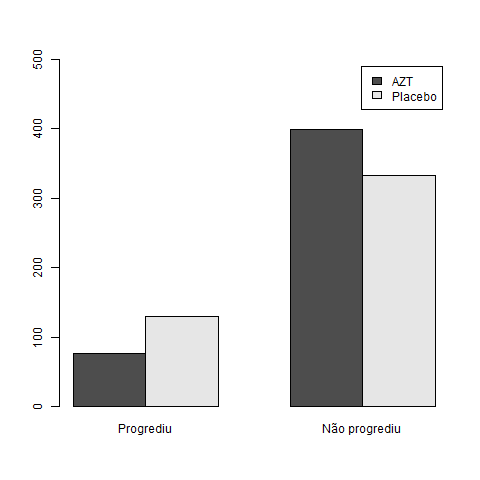
\includegraphics[height=\textheight]{Cap26-27/barplot}
  \end{center}
\end{frame}

\begin{frame}{Visualização - pizza}
  \begin{block}{Atenção}
    NÃO use gráfico de pizza!
  \end{block}
  \begin{itemize}
    \footnotesize
  \item É uma visualização ineficiente
  \item Nosso olho é ``bom'' para julgar distâncias/comprimentos
  \item Nosso olho é ruim para julgar áreas
  \item Indicado {\bf apenas} quando as categorias são muito discrepantes
  \end{itemize}
  \begin{block}{Cleveland (1985)}
    \small
    {\em ``Data that can be shown by pie charts always can be shown by a dot chart.

      This means that judgements of position along a common scale can be made instead of the less accurate angle judgements.''}
  \end{block}
\end{frame}

\subsection{Resumo}

\begin{frame}{Resumo}
  \begin{itemize}
  \item O teste exato de fisher é um teste de independência entre os grupos
  \item O teste Qui-quadrado é uma boa aproximação, para N grande
  \end{itemize}
\end{frame}

\section{Aprofundamento}

\subsection{Aprofundamento}

\begin{frame}{Aprofundamento}
  \begin{block}{Leitura obrigatória}
    \begin{itemize}
      \footnotesize
    \item Capítulo 26.
    \item Capítulo 27, pular a seção: Calculando o poder
    \end{itemize}
  \end{block}
  \begin{block}{Leitura recomendada}
    \begin{itemize}
      \scriptsize
    \item Capítulo 29: Outros testes de tabelas de contingência
    \item Capítulo 27, seção: Calculando o poder
    \end{itemize}
  \end{block}
\end{frame}

\end{document}
